\subsection{Propuesta de solución}
Se plantea el desarrollo de un prototipo de sistema de monitoreo y control para
la gestión eficiente del consumo de agua en los cultivos de plantas del Vivero
Michita, empleando lógica difusa. Este sistema permitirá a
los responsables del vivero supervisar y regular el riego de manera precisa y
adaptativa, optimizando así el uso del recurso hídrico en las áreas de cultivo.
Como se muestra en la Figura \ref{fig:esquema_riego}, el diagrama de procesos
del sistema es fundamental para comprender su estructura.

\newpage

\begin{figure}[h]
    \centering
    \makebox[\textwidth]{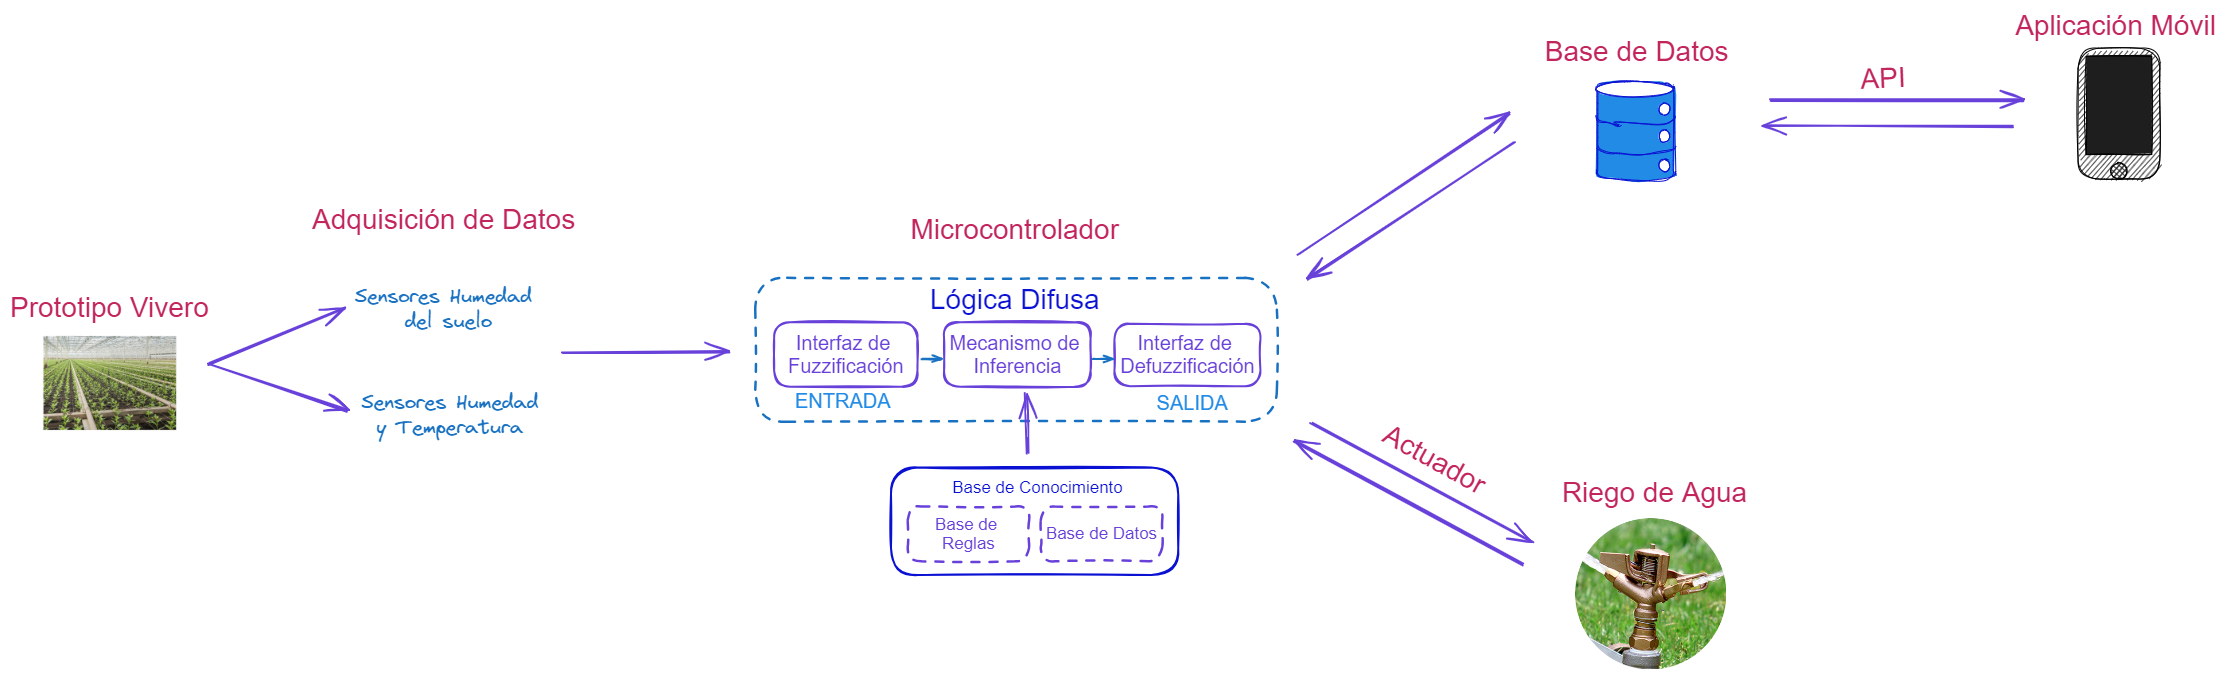
\includegraphics[width=15cm,height=30cm,keepaspectratio]{resources/images/ESQUEMA.png}}
    \caption{Esquema del sistema}
    \label{fig:esquema_riego}
\end{figure}


Se emplearán diversas herramientas tecnológicas. Es por ello que se utilizará
sensores de humedad del suelo, temperatura y ambiente que proporcionaran
información en tiempo real sobre las condiciones del vivero. Con el apoyo de un
controlador, estos datos permitirán ajustar el riego de manera precisa y
eficiente. \bigbreak La lógica difusa se utilizará para adaptar las estrategias
de riego a los cambios ambientales del vivero, optimizando así el uso del agua.
La información recolectada por los sensores será analizada en una base de
datos, brindando datos valiosos para mejorar el manejo del agua en el vivero.
\bigbreak La API se encargar de que las aplicaciones móviles se conecten
fácilmente con los datos de los sensores. Esta conexión permitirá que la
información recopilada por los sensores, como datos de humedad y temperatura,
sea accesible en las aplicaciones. De esta forma, los encargados del vivero
podrán usar la aplicación móvil para tomar decisiones sobre el riego, basándose
en estos datos en tiempo real. Este enfoque tecnológico, combinado con la
lógica difusa que adapta las estrategias de riego, será clave para mejorar
eficazmente el sistema de riego en el vivero.

% \bigbreak
% Es por ello que, la propuesta se destaca por su enfoque innovador que es el uso de la lógica difusa para el desarrollo del sistema de monitoreo y control del consumo de agua. Esta técnica de inteligencia artificial permite tomar decisiones a partir de valores imprecisos, adaptándose a las condiciones cambiantes del entorno, como las condiciones climáticas y las necesidades de las plantas.